%Import the Thesis formatting
\documentclass[12pt]{ucthesis}

%Package Imports
\usepackage[pdftex]{graphicx}
\usepackage{parskip}


\begin{document}
\title{Improvements and Analysis of Software Based 1200 Baud Audio Frequency Shift Keying Demodulation}
\author{Robert Campbell}
\degreemonth{June} \degreeyear{2014} \degree{Master of Science}
\defensemonth{June} \defenseyear{2014}
\numberofmembers{3} \chair{John Bellardo, Ph.D.} \othermemberA{Bridget Benson, Ph.D.} \othermemberB{Dennis Derickson, Ph.D.} \field{Computer Science} \campus{San Luis Obispo}
\copyrightyears{seven}
\maketitle

\begin{frontmatter}

\copyrightpage

\committeemembershippage

\begin{abstract}
Digital communications continues to be an interesting field of study as new technologies appear and old methodologies get revisited or renovated. The goal of this research was to look into the old digital communication scheme of Bell 202 and find a way to demodulate the signal in software with results similar to those of hardware demodulators. The research shows that through using Sivan Toledo’s JavaAX25 software package, new demodulation algorithms can be implemented that decode Bell 202 AX.25 encoded packets that the existing software tool could not.
\end{abstract}


\tableofcontents

\end{frontmatter}

\chapter{Introduction}

Amateur Radio Operators, commonly referred to as "hams," make the best of resources available to them. However, once something is working a "don't touch it if it ain't broke" approach is often taken. Between these two mentalities some interesting phenomenon have occurred within the ham community. For example, some radio systems that are in active service today have only seen very minimal attention since the 1980's when they were originally installed. The implementation and development of the Automated Packet Reporting System (APRS) is no exception to the way hams approach things\,\cite{Bruninga}. Much of this system is based off older hardware and protocols - from the 1980s - that was readily available and few improvements have been made. Unfortunately, although the specification has been relatively stable there are inconsistencies. These inconsistencies include varying implementations from vendor to vendor as well as portions of the specification that are not clearly defined resulting in vastly inconsistent performance\,\cite{KWFThesis, KWFTAPR}.

So, what is APRS, and why does it matter? A brief introduction to APRS is that it is a digital communication scheme used by hams where a packet (whose content is varied, but is usually a GPS position - which is what gave APRS it's original name "Automated Position Reporting System"\cite{WikiAPRS}) is sent out over radio and then interpreted by other receiving stations. Figure \ref{APRSEndToEnd} shows one example of an end to end APRS system. A major challenge to this protocol and many other method of digital communication is the fact that it uses radio. Transmitting the signal wirelessly over radio means that it is susceptible to interference, weak signals as the distance from the transmitting station increases, as well as a myriad of other items. This research focuses specifically on the receiving end of these signals in order to see what improvements can be made to software based approaches to demodulating (decoding) these packets, which is represented by the TNC block in Figure \ref{APRSEndToEnd}. However, to more accurately portray software based demodulation the TNC block in the figure should be moved inside of the computer block since the receive radio audio is passed straight to the computer and then interpreted by this special software.

\begin{figure}
  \centering
	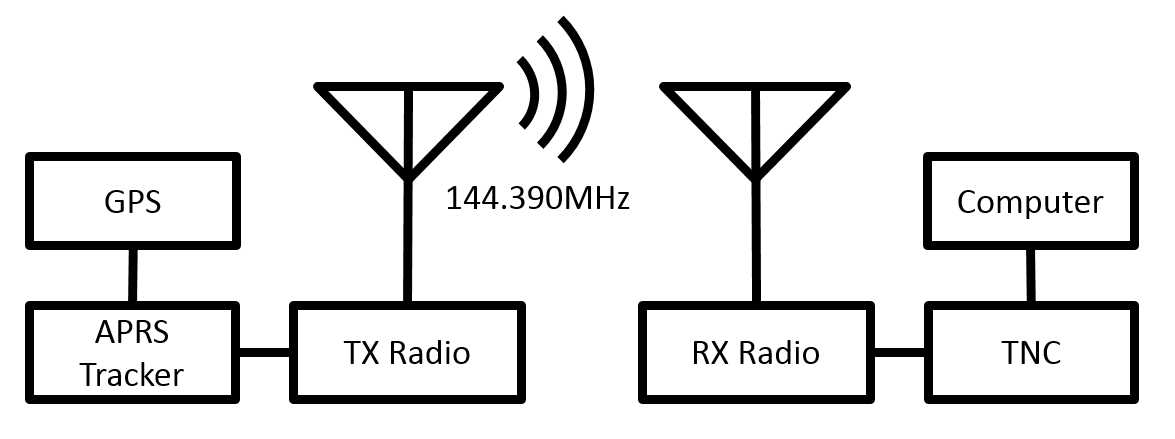
\includegraphics[width=0.75\linewidth]{images/APRSEndToEnd.PNG} 
   \caption[Block diagram of an example APRS system end to end.]{Block diagram of an example APRS system end to end. The GPS communicates information using NEMA to the APRS tracker, the tracker then takes this information and the preferences in its configuration to formulate APRS packets. The APRS packets are encoded by the tracker and the resulting audio passed to a transmit radio which sends the data. Typically this is done on frequency 144.390MHz in the United States. Receiving radios tuned to the same frequency pass the received audio to a TNC which decodes the packet and passes it to a computer using RS-232.}
   \label{APRSEndToEnd}
\end{figure}

The reasoning for trying to make improvements in software based demodulation are many, but a few of the more motivational ones are to follow. One advantage of doing software based demodulation is that it removes the necessity of specialty hardware; Instead of having dedicated hardware whose sole purpose is to modulate and demodulate APRS packets, hams can use a computer to do these tasks. By using a computer's sound card, audio from the radio can be processed using software to decode received packets, or audio can be played from the sound card to the radio to be transmitted. With the abundance of personal computers, this can provide a much cheaper solution for hams who are interested in trying out APRS without having to put down a potentially big initial investment (\textasciitilde\$200\,\cite{Kantronics2014,Outlet2014}) for a piece of hardware that serves one purpose. The price of this specialty hardware is steep and it is limited to only performing communication on a single channel. When using a line in / out on a computer they are typically stereo, meaning that a single sound card could handle operations on multiple channels. If two channels just is not enough the capabilities of a computer demodulator can be expanded by merely adding another sound card which is relatively cheap at \textasciitilde\$20\,\cite{Newegg}. See Table \ref{costCompareTable} for a comparison of the cost for hardware and software. From the table it can be seen that the cost to perform communication on 4 channels using dedicated hardware the cost would be \$800! For this cost a whole computer with a half dozen sound cards could be purchased, only further expanding capabilities.

\begin{table}
	\begin{center}
		\begin{tabular}{ | l | r | r | r | r | }
		\hline
			Cost for: & 1 Channel & 2 Channels & 3 Channels & 4 Channels \\ \hline
			Software & \$0 & \$0 & \$20 & \$20 \\ \hline
			Hardware & \$200 & \$400 & \$600 & \$800 \\
			\hline
		\end{tabular}
		\caption[Hardware and Software Cost Comparison]{Cost comparison of conducting APRS communications on 1 through 4 channels for hardware versus software assuming the user already owns a computer.}
		\label{costCompareTable}
	\end{center}
\end{table}

In addition to the the price advantages of software based demodulation approaches, there is also one other primary advantage. If software is being used instead of hardware there is the potential for a lot more capabilities since processing power and available memory increase drastically. For instance, one of the dedicated hardware solutions, the Kantronics KPC-3 Plus, has a mere 512KB of memory compared to that of any computer which is over 4GB as of 2014 - and that is just the ram, not hard drive space\,\cite{Kantronics2014,Graham-Smith2014}. Additionally, instead of just being able to handle live events and process each data point in the best manner possible as soon as it comes in, post processing becomes an option.

With the cost and versatility of a software demodulation solution now introduced, the paper addresses the following: Chapter 2 goes into background information, with a deeper introduction to APRS and a presentation of the aspects important to understanding this research. In Chapter 3, some of the current methods for interfacing with APRS, both hardware and software, are explained. Demodulation techniques are discussed in Chapter 4. Chapter 5 talks about the challenges of demodulating APRS packets. Chapter 6 discusses the methods used for benchmarking and comparing the demodulators. In Chapter 7, information on how the demodulators and algorithms are tested is presented. Chapter 8 goes into more detail about the software implementations in this project. Chapter 9 discusses the results of both the newly implemented algorithms and compares them to other demodulators. Areas of additional research and future work are discussed in Chapter 10. Chapter 11 is concluding remarks.

\chapter{Background}

APRS is a local area awareness network designed from hams (amateur radio operators), by hams. There is a plethora of features supported within the specification of APRS including the sending of messages, bulletins, meteorological data, waypoints, objects, and most commonly GPS locations. Many of the capabilities have not been fully implemented and other implementation details are inconsistent. The goal of this research is not to discuss the shortcoming in the APRS protocol itself which lies within its implementation and use on top of the AX.25 protocol. Instead this research focuses on Layer 1 problems in the Open System Interconnection (OSI) model. 
The Layer 1 protocol for ARPS is based off of a Bell 202 modem. The Bell 202 modem was patented in 1984 using 1200Hz and 2200Hz tones, although the patent was originally filed in 1981 [1]. Interestingly, the international telecommunication union didn’t publish a standard for these modems that were used in telephone networks until 1988. In the standard, however they use 1300Hz and 2100Hz tones for symbol 1 (called a mark) and symbol 0 (called a space) respectively [2]. The basic modulation scheme is that the marks and spaces are used in a non-return to zero inverted (NRZI) encoding for the actual data. When a transition occurs from one symbol to another that symbolizes a ‘0’ bit in the original data bit stream and if the symbol remains constant over multiple symbol periods, that signifies a ‘1’ bit in the original data bit stream. It is also worth noting that there will be no more than 5 consecutive symbols during a packet, as the scheme will bit stuff in order to make sure that synchronization on the clock can be maintained. The only exception to this rule is for the flag(s) that mark the start and end of a packet. The AX.25 flag is hex 0x7E without bit stuffing. Common practice is to send multiple flags consecutively to give transmitting radio time to key up and settle and to give receiving radios time for their squelch to open.
This encoding and modulation is used to transmit the data of the APRS packets, but further background is needed in the APRS environment to discuss where this research applies. As mentioned this will not be looking into the APRS protocol itself but more focused on the Bell 202 modem and specifically the demodulation aspects. Implementing a Bell 202 modulator is simple in comparison to making a robust demodulator - especially when trying to implement one in software.

\section{Hardware Based Demodulators}

Currently there are many systems that will demodulate these Bell 202 encoded APRS packets. The original hardware used for this communication style was dedicated modems similar to dial-up 56k modems that did the encoding and decoding. These modems were connected directly to the radio and the radio would let the modem know through a signal pin if it was receiving what it thought was a data carrying signal. The terminal node controller (TNC), a modem used in AX.25 operation, would let the radio know by signaling the radio to transmit when it had data to send out. As mentioned in the introduction and early in this section, the technologies that are being used for this data transport originated in the late 1980s even though the spec for the protocol itself did not get officially released until 2000. This serves as a reminder that old hardware is commonly used that is not well understood. If a user gets something reasonable working, they will use it without doing a full analysis on edge cases or making simple modification to improve performance.
With a radio and a Terminal Node Controller, digipeaters (digital packet repeaters) are possible. Within the testing scope of this project there are two TNCs that used in order to be able to compare our results to them which were the AEA PK-88 and the Kantronics KAM Plus. Digipeaters are an essential part of the ham packet network, but many users wish to report their GPS position onto the APRS network instead of just relaying traffic for other stations. In order to accomplish this, a GPS receiver is required. Now, stations can take the data from their GPS receiver and put it in the payload of the APRS packet and transmit the GPS reported position onto the network. However, the PK-88 and the KAM Plus although used very frequently in APRS systems are not fully dedicated hardware for APRS, but instead modems that are being used for ARPS.

\section{Dedicated Hardware}

Many people know exactly what they would like to do with APRS and exactly what traffic they want to contribute to the APRS network. This has initiated dedicated hardware for APRS with a UI in order to make it simple for the end users to quickly run and configure their APRS stations. Some examples of APRS exclusive devices are ArgentData’s OpenTrackers, Byonics’ TinyTrack, and Fox Delta’s Fox Track. These compact packages along with a radio and a GPS module perform APRS tasks at a satisfactory level for many users.
Since the average user only wants to report positional information, these dedicated devices make it simple to setup. These trackers contain many features, but they don’t implement the full APRS specification. An example is the messaging service since these devices don’t have a display for the message. Certain radio manufacturers have begun to integrating the TNCs into the radios themselves to utilize the radio’s screen. The Kenwood TM-D700 series and Yaesu FTM-350 are examples.
However, both the options that were presented in section 2.1 and 2.2 require going out and buying special hardware in order to perform APRS. This can be expensive and cost prohibitive for some hams to be able to begin APRS operations.

\section{Software Based Demodulators}

It can be assumed that before a ham operator becomes interested in the APRS network and sending APRS packets that they will already have a radio. So, if they already have a radio all they have to do is buy a piece of hardware that will do the modulation in order to send a packet. However, hardware costs money and as hams are at least somewhat technology savvy most have computers. A software solution seeks to take advantage of the computer already in the operator’s possession to do the modulation and demodulation and hence offer a cheaper alternative.
This seems to be a route that some are taking and a demodulation scheme that this project explores in detail, but first some more information on current systems that operate in this software realm. Some examples of the software that can be used are George Rossopoylos’s Packet Engine or Thomas Sailer’s Linux Sound Modem. On a computer, even ones with minimal resources, there are algorithms that are being used to demodulate the APRS packets. Again, what this project aims to investigate is if improvements can be made to the algorithms used to decode these packets in order to make the software based systems more robust and as good as dedicated hardware. Preliminary testing shows that the software still has room for improvement in order to be at least as good as dedicated hardware.


\end{document}
